%% OfficeFloor - http://www.officefloor.net
%% Copyright (C) 2013 Daniel Sagenschneider
%%
%% This program is free software: you can redistribute it and/or modify
%% it under the terms of the GNU General Public License as published by
%% the Free Software Foundation, either version 3 of the License, or
%% (at your option) any later version.
%%
%% This program is distributed in the hope that it will be useful,
%% but WITHOUT ANY WARRANTY; without even the implied warranty of
%% MERCHANTABILITY or FITNESS FOR A PARTICULAR PURPOSE.  See the
%% GNU General Public License for more details.
%%
%% You should have received a copy of the GNU General Public License
%% along with this program.  If not, see <http://www.gnu.org/licenses/>.
%%
%% While this document is not a program, it conveys the underlying design 
%% of OfficeFloor (it is the expression of how to implement the ideas of 
%% Thread Injection, Implicit Thread, Continuation Injection, Operation 
%% Orchestration, Inversion of Control) and as such any program derived from 
%% the contents (expression) of this document is considered conveying 
%% (copying/modifying) the OfficeFloor expression and is therefore subject 
%% to the licensing of OfficeFloor.




%%This is a very basic article template.
%%There is just one section and two subsections.
\documentclass[prodmode]{style/acmlarge}

% Include packages
\usepackage{listings}
\usepackage{caption}


% Metadata Information
\acmVolume{V}
\acmNumber{N}
\acmArticle{A}
\articleSeq{S}
\acmYear{YYYY}
\acmMonth{0}

% Package to generate and customize Algorithm as per ACM style
\usepackage[ruled]{style/algorithm2e}
\SetAlFnt{\algofont}
\SetAlCapFnt{\algofont}
\SetAlCapNameFnt{\algofont}
\SetAlCapHSkip{0pt}
\IncMargin{-\parindent}
\renewcommand{\algorithmcfname}{ALGORITHM}

% Page heads
\markboth{D. Sagenschneider}{Software Design based on Patterns within an Office}


\title{Software Design based on Patterns within an Office}
\author{DANIEL SAGENSCHNEIDER \affil{OfficeFloor, daniel@officefloor.net}}

\begin{abstract}
OfficeFloor is a middleware framework that is architected from the patterns
occuring within an office.  Using the proven patterns from the office has
provided improved performance tuning and reduced coupling over existing software
design patterns for middleware frameworks.  Furthermore, the patterns have
provided inversion of control to build applications bottom-up.  This bottom-up
approach to building applications better suits modern development methodologies,
such Agile, that evolve the application's architecture upwards.
\end{abstract}

\category{}{}{}[]

\terms{Design, Performance, Standardization}
\keywords{Implicit Thread, Inversion of Control, Task Orchestration}

\acmformat{Sagenschneider, D. 2013.Software Design based on patterns within an Office.}

\copyr{Copyright 2013 is held by the author}

\begin{document}

% Configure Graphics package
\graphicspath{{./pdf/}}
\DeclareGraphicsExtensions{.pdf}

% Configure Listings package
\lstset{language=Java}

% Configure Captions package (listing small font)
\captionsetup[lstlisting]{font=footnotesize}


\begin{bottomstuff}
This work is the result of the author's development of OfficeFloor.\\
Author: D. Sagenschneider; email: daniel@officefloor.net\\

Permission to make digital or hard copies of all or part of this work for
personal or classroom use is granted without fee provided that copies are not
made or distributed for profit or commercial advantage and that copies bear this
notice and the full citation on the first page. To copy otherwise, to republish,
to post on servers or to redistribute to lists, requires prior specific
permission. A preliminary version of this paper was presented in a writers'
workshop at the 18th European Conference on Pattern Languages of Programs
(PLoP).
\end{bottomstuff}

\maketitle


%% TODO before final draft:
%%   - confirm SEDA adds/removes threads
%%   - go through GOF to confirm any alternate names

\section{Introduction}

OfficeFloor~\cite{officefloor} is a middleware framework that models its
architecture on patterns occuring in offices.

The premise of this modelling is that business processes occurred manually
within an office before technology systems began automating tasks.  The manual
office processes are accepted by people and the patterns proven within many
business organisations.

This paper discusses these office patterns and how they remove constraints
within existing software design patterns.  The patterns presented are the
patterns used by OfficeFloor in its implementatation as a middleware framework.
Usage patterns for developers to build applications with OfficeFloor is left to
future work.

To be able to relate the office patterns to software design patterns the
following analogies are made:
\begin{description}
  \item[Thread] is mapped to the concept of a Person (Worker),
  \item[Method] is the functionality of a Task (particular step of a process),
  \item[Object fields] is the structured information managed within an office (e.g. form).
\end{description}

The patterns presented in this paper are discussed in three sections.  The first
section presents the patterns for execution of tasks.  The second section
presents patterns for co-ordination of tasks.  The third section presents
patterns for building processes from tasks.  Each section is written in two
parts.  The first part will list the office patterns and how they influence
change in the software design.  The second part of each section provides notes
on implementation.  This paper assumes knowledge of existing software design
patterns only for the implementation notes within each section.  The
implementation notes may be skipped by those readers only interested in the
influence of the office patterns on software design.



\section{Patterns for execution of tasks}

The following patterns model the execution of methods after the way tasks are
undertaken within an office.  The implementation notes at the end provide
details on how to implement the combined patterns.


\subsection{\textsc{\textbf{team}}}

\subsubsection*{Alternate name} \textsc{thread pool} \cite{thread-per-request}.

\subsubsection*{Context} Within an office work loads can be far above that
possible by a single person. This is resolved within an office by creating a
team of people to concurrently undertake the tasks.

Developers write code of a method (task) for a single thread (person).

\subsubsection*{Problem} Improving throughput of executing many single threaded methods.

\subsubsection*{Forces} Developer writes intuitive sequential code.

\subsubsection*{Solution} Use a pool of threads to execute the tasks
concurrently.

\subsubsection*{Consequences} Having more people allows getting more work done.
Similarly having more threads allows more tasks to be executed.

The people in the office need to coordinate so the tasks get done correctly and
efficiently.  This is similar of the concurrency issues occurring in executing
methods concurrently.

\subsubsection*{Notes} See the \textsc{thread pool}
pattern~\cite{thread-per-request} for a detailed explanation.  The \textsc{team}
pattern is provided as an example to highlight how the analogies in the
introduction may enable re-use of office patterns.



\subsection{\textsc{\textbf{categorise task}}}

\subsubsection*{Context} To assign a task to a particular team when there are multiple teams, a
description of the task is required to identify which team is responsible for
undertaking the task.  This description allows categorising similar tasks
together to be undertaken by a particular team for improved efficiencies.  For
example, a financial task should be undertaken by the finance team.

\subsubsection*{Problem} Can the method provide a description of itself for being categorised into a group?

\subsubsection*{Forces} The method name is free text and is unlikely to follow a naming convention that
allows parsing out a category.

The developer should not have to write the description of the method.

\subsubsection*{Solution} Use the parameter types of the method to categorise
the method.  For example, all methods that declare a database connection
parameter can be grouped into a category of tasks that are likely to interact
with the database.

For finer grained categorisation, annotations of the parameter types may also be
used.

\subsubsection*{Consequences} The method name is not required for categorising.

The developer is not required to provide any more details except the parameters
the method requires.

Methods that have unused parameters may be incorrectly categorised.

\subsubsection*{Related Patterns}

\textsc{responsible team} provides the particular teams to execute the
categorised methods.



\subsection{\textsc{\textbf{responsible team}}}

\subsubsection*{Context} To accomplish the process, there are different teams
responsible for differing tasks in the process.  For example, the financial team
will do the finance tasks and the software development team will do the coding
tasks.

Having this split in responsibility over the categorised tasks allows
specialising the team to their tasks.

\subsubsection*{Problem} Making the \textsc{thread pool} responsible for a
particular category of methods.

\subsubsection*{Forces} The possibly configured thread pool name is free text
and is unlikely to follow a naming convention that allows parsing out its
responsible task categories.

The developer should not have to provide code to make decisions over thread pool
responsibilities.

\subsubsection*{Solution} Configure each thread pool with an attribute
containing the type(s) that defines its responsible category(s).  Methods are
then executed by matching on their parameter types (\textsc{categorise task}
types) against the configured thread pool responsibility type.  A default thread
pool is used if no match occurs.

For example, configure the thread pool responsible for all database interaction
with the database connection type.  As each method is categorised by the
\textsc{categorise task} pattern, all methods requiring a database connection
are executed by this thread pool.

\subsubsection*{Consequences} There will always be a thread available in each
thread pool to execute their respective responsible tasks.  Subsequently, if
there is a significant increase in the number of tasks in one category all
threads do not become focused on these tasks to the detriment of the other
categories of tasks.

Threads of the thread pool may be specialised (e.g. change in nice value,
affinity to CPU) based on the responsibilities of their thread pool.  Threads
may, however, be idle if no tasks occur for their responsible task category.

\subsubsection*{Related Patterns} Is a sequence on the \textsc{team} to identify
responsible categories of tasks to execute.



\subsection{\textsc{\textbf{manage team size}}}

\subsubsection*{Alternate name} Adaptive Resource Management \cite{seda}. 

\subsubsection*{Context} As the number of tasks for a responsible team grows or
shrinks, the size of team is altered to obtain optimal throughput.  For example,
near the end of the financial year the finance team may be increased in size for
the additional number of financial year end tasks.  The software development
team, however, would not be changed in size as the development tasks would stay
the same in number.

\subsubsection*{Problem} Obtain optimal throughput execution of methods by a
thread pool.

\subsubsection*{Forces} Having too few threads will under utilize the hardware
and not provide optimal throughput.  Having too many threads will cause
excessive thread context-switching and exhaustion of available resources (e.g.
memory) which will decrease throughput.

\subsubsection*{Solution} As each thread pool is responsible for particular
dependency (resource), use adaptive resource management~\cite{seda} to manage
the number of threads within each thread pool.

Adaptive resource management (from the Staged Event Driven Achitecture
\cite{seda}) monitors the number of tasks and their execution time and
adds/removes threads to achieve optimal throughput.

\subsubsection*{Consequences} The thread pool size will dynamically grow/shrink
based on its load of responsible methods to execute.  This, however, does
require a small overhead in monitoring the execution of methods.



\subsection{\textsc{\textbf{do it yourself}}}

\subsubsection*{Alternate name} \textsc{reactor}~\cite{reactor}.

\subsubsection*{Context} Certain tasks are more efficient to be undertaken
yourself without having to assign to another team.  If every task along the
process had to be undertaken by a different team, it would create significant
communication overheads that would negatively impact the efficiency of the
office.  Therefore, within an office many tasks are undertaken by the current
person involved in the process.

Assigning a method to a thread pool requires one or more thread context
switches.  Having to thread context switch for each method call is inefficient
and will degrade performance of the application.

\subsubsection*{Problem} Avoid context switch in executing certain methods (tasks).

\subsubsection*{Forces} Each category of methods will be executed by a particular
responsible thread pool.  Stepping between these categories causes different
responsible thread pools to be used that requires to thread context-switch between
each task category switch.

\subsubsection*{Solution} Use a responsible thread pool that has no threads and
uses the thread of control that registers the method with the thread pool to
execute the task.

\subsubsection*{Consequences} Categories of methods may be executed by the
current thread of control and not incur a thread context-switch to be executed
by another thread pool.

\subsubsection*{Related Patterns} Is a sequence on the \textsc{responsible team}
to reduce thread context-switching.



\subsection{\textsc{\textbf{team too busy}}}

\subsubsection*{Alternate name} Admission Control \cite{seda}. 

\subsubsection*{Context} Teams may not be able to complete all tasks within the
required period of time.  The teams may be increased in size to cope with the
additional tasks.  However, at a certain point there are too many tasks and to
cope the team will not take on new tasks.

The thread pool queues methods for execution when all threads of the pool are
exhausted.  At a certain point the queue becomes too long that new methods added
to the queue will not be executed within a reasonable period of time.

\subsubsection*{Problem} Stop the thread pool taking on new methods so it may
cope with the current load of methods.

\subsubsection*{Forces} The thread pool will sequentially execute all methods
added to its queue.  When the number of methods registered for execution is
continually more than the number of methods able to be executed, the queue
grows.  At a certain point the time between registering a method and the actual
execution of the method is so far apart that the resulting method execution is
no longer relevant.  Execution of these methods then results in wasted use of
threads.

\subsubsection*{Solution} At a certain queue size, cancel further methods from
being registered.

\subsubsection*{Consequences} The thread pool will able to execute methods that
are registered. For methods not registered, alternate tasks are undertaken by
another less busy thread pool.

At high loads of methods some methods will not be executed.  This, however,
allows the thread pool to execute the methods it can in a timely manner.

\subsubsection*{Related Patterns} Uses \textsc{escalation} to handle cancelled
methods.



\subsection{Implementation of the task execution patterns}

\subsubsection*{Background}

Both the \textsc{thread-per-request} pattern \cite{thread-per-request} and the
\textsc{proactor} pattern \cite{proactor} enable a different thread of control
for the execution of a request/component.  These patterns allow for concurrent
execution by utilising many threads.  For efficiencies the \textsc{Thread Pool}
pattern \cite{thread-per-request} is commonly used to pool threads to reduce
thread management overheads.

As identified by the \textsc{proactor} pattern, the threading ``must be designed
carefully to support prioritization and cancellation'' \cite[p. 8]{proactor} of
the execution of components.  Both the \textsc{thread-per-request} pattern and
the \textsc{proactor} pattern, however, do not define algorithms for
prioritisation and cancellation of components and leaves this to the developer.

Performance analysis of web servers identifies the importance of this
prioritisation tuning
\cite{tuning-important,low-server-footprint,tuning-os-important}.
Serving static web content follows a similar sequence of tasks making the use of
a pool of threads sufficient.  In contrast, servicing dynamic content has
significantly varying tasks.  Utilising a pool of threads to service all dynamic
content tasks can result in tuning trade-offs that may result in performance
degradation of the server during particular load profiles (e.g. high load of
requests for database data that are starving requests for cached data of a
thread).  Better isolation of tasks is necessary to reduce trade-offs in
performance tuning.

Having an ability to cancel tasks is important to avoid overloading.  As
load increases on the server, the resources available will be exhausted causing
delays in servicing requests and in some scenarios cause the server to crash
(e.g. exhausting available memory).  Tasks must be able to be cancelled to
reduce the load on the server.  However, only tasks causing bottlenecks
should be cancelled (e.g. a request for cached data should not be cancelled if
it is the database that is overloaded).


\subsubsection*{Implementation}

The task is the object that wraps the method to provide a standard interface for
execution of the method.  This enables for a single \texttt{TaskExecutor}
(Listing \ref{lst:TaskExecutionInterfaces}) implementation to execute
differing methods.

To invoke a method, the client code invokes \texttt{executeTask(\ldots)}
(Listing \ref{lst:TaskExecutionInterfaces}) with the identifier of the desired
task along with an argument for a parameter of the task.  Figure
\ref{fig:ExecuteComponentSequenceDiagram} provides a sequence diagram of
executing a task.  The \texttt{TaskExecutor} uses the
\texttt{DependencyInjectionFactory} to construct the appropriate \texttt{Task}
and then assigns it for execution by one of the many developer configured thread
pools (\textsc{team}).

\lstset{caption=\textsc{thread injection} pattern interfaces\protect\footnotemark.}
\begin{lstlisting}[float,label=lst:TaskExecutionInterfaces]

    interface Task {
        void execute(Object parameter); 
        void cancel(Object parameter, Exception cause);
    }

    interface TaskExecutor {
        void executeTask(String taskId, Object parameter);
    }

    interface DependencyInjectionFactory {
        Task createTask(String taskId);
        Type[] getRequiredDependencyTypes(String taskId);
    }
\end{lstlisting}
\footnotetext{An example implementation of the
\texttt{DependencyInjectionFactory} is wrapping Spring's \cite{spring}
\texttt{DefaultListableBeanFactory} to implement
\texttt{createComponent(\ldots)} by calling \texttt{getBean(\ldots)} and
implement \texttt{getRequiredDependencyTypes(\ldots)} by recursively calling
\texttt{getBeanDefinition(\ldots)}/\texttt{getDependsOn()} to create the 
list of types.}


\begin{figure}[!t]
\centering
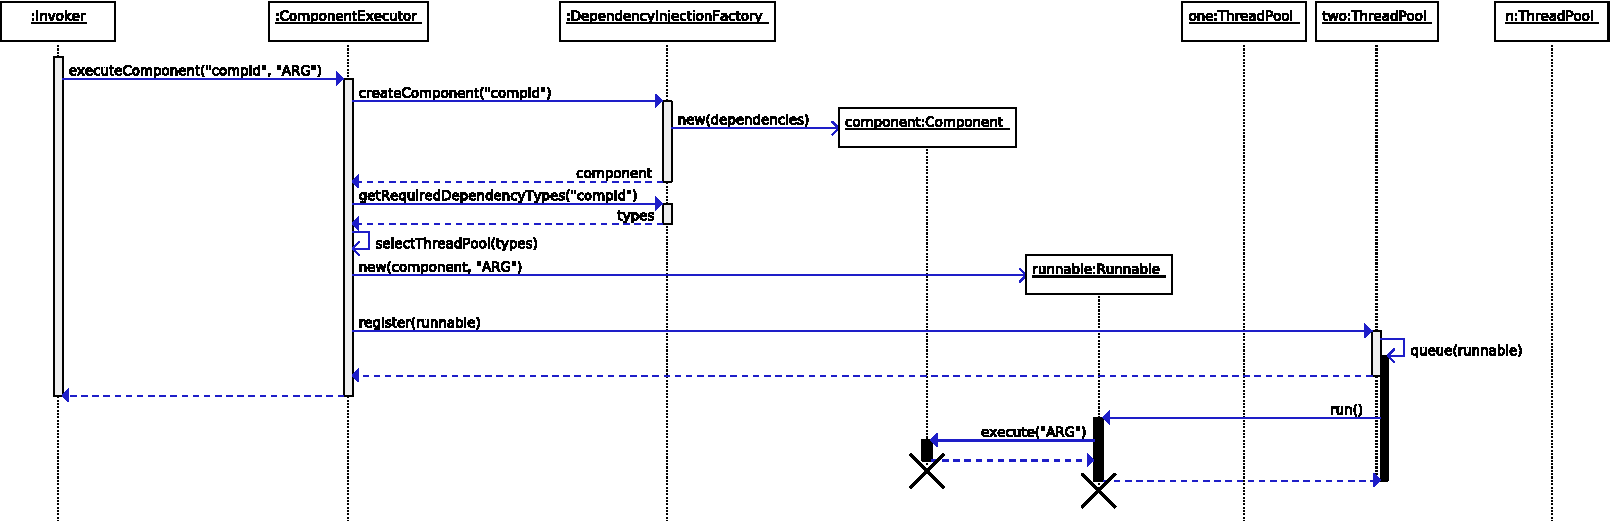
\includegraphics[width=6in]{ExecuteComponentSequenceDiagram}
\caption{Sequence diagram of invoking \texttt{executeComponent(\ldots)}.}
\label{fig:ExecuteComponentSequenceDiagram}
\end{figure}

The prioritisation is achieved by the
\texttt{getRequiredDependencyTypes(\ldots)} method providing the extrinsic
\textsc{dependency injection} \cite{ioc} meta-data for the task
\footnote{\textsc{dependency injection} frameworks using qualification to
identify dependencies of the same type may return a type object containing both
class and qualifier rather than just a class.  The thread pool matching may then
incorporate the qualifier.}.  The developer configures one or more thread pools
responsible for tasks with a particular type of dependency\footnote{Thread pools
may be associated with more than one dependency type.}.  The task is then
matched by its required dependency types (\textsc{categorise task}) to a thread
pool responsible for one or more of its dependency types (\textsc{responsible
team})\footnote{The \texttt{taskId} may also be used for very fine grained
mapping.}.  The \texttt{execute(\ldots)} method (Listing
\ref{lst:TaskExecutionInterfaces}) is then invoked by a thread from the
matching thread pool to execute the task (and its contained method). This
provides the necessary isolation of differing tasks for improved tuning of the
server.

For tasks not having dependencies (nor dependencies of any performance
significance), a default thread pool is configured by the developer for their
execution.  This ensures all components are mapped to a thread pool.  It also
means that thread pools need only be configured for dependencies requiring
isolation. \textbf{TODO: pattern for this paragraph}

To achieve further efficiencies the implementation of each thread pool may be
specific to its responsible dependency type.  For example, the thread pool may
contain multiple threads for concurrent execution of tasks with threads
added/removing based on the load of tasks (\textsc{manage team sizes}), a single
thread for serial execution of tasks (\textbf{TODO design pattern for this}), or
no threads and execute components by borrowing the thread to reduce
thread-context switching (\textsc{do it yourself}).

The \texttt{cancel(\ldots)} method (Listing \ref{lst:TaskExecutionInterfaces})
provides means for the \texttt{TaskExecutor} to cancel the task.
The \texttt{TaskExecutor} will cancel new tasks for a particular thread pool
when queuing the task for a thread will result in exceeding a particular
threshold\footnote{A sufficient threshold would be ensuring the wait time,
determined by a running average of execution time multiplied against the number
of components currently in the queue, is below a certain time.} (\textsc{team
too busy}).  Each thread pool may have its own thresholds particular to its
responsible dependency types.  As tasks are mapped to particular thread pools,
this ensures only the appropriate tasks are cancelled.

Once cancelled, the \texttt{TaskExecutor} may discard the task.  The
implementation of the \texttt{can\-cel(\ldots)} method is covered in the
\textsc{escalation} pattern.


\subsubsection*{Consequences}

The isolation provided by using multiple thread pools enables improved tuning of
the server.  Tuning the thread pools (such as restricting the number of threads
or changing the pool's thread nice values) allows prioritising threads and
subsequently prioritising groups of related components.

As each thread pool is executing components for a particular dependency (or set
of dependencies), this allows for adaptive resource management and admission
control regarding the dependency \cite{seda}.  This enables both the number of
threads and dependencies to be dynamically altered to improve throughput.
However, when maximum throughput is reached additional components for execution
above this threshold can be cancelled.

To improve performance of runtime decisions the mapping of component to thread
pool may be cached.  As the dependencies for each component is static, at
application start up time the \texttt{TaskExecutor} may preprocess and
cache the mapping of \texttt{Task} to thread pools to reduce runtime
decision overheads.  This pre-mapping of tasks may also provide warnings
where dependencies of a task make it possible to map the task to
multiple thread pools.  Different conflict mapping resolutions may be employed,
however, ordering the thread pools and assigning tasks based on first match
is a sufficiently adequate algorithm.

For low load servers where a single thread pool is sufficient, having multiple
thread pools can cause increased complexity for developer configuration.  While
this provides the flexibility to focus the tuning of isolated categories of
tasks by tuning their mapped thread pool, it does put the burden on the
developer to understand thread related performance issues (e.g. costs related to
thread stack memory and thread-context switching) and the performance of the
dependencies (along with their related tasks).

The implementation looses its ability to effectively prioritise and cancel tasks
if the task dependencies are too similar.  For example, when used with the
\textsc{thread-per-request} pattern within a web server, all request handling
for dynamic content is likely to use a database connection.  While this will
allow isolation of requests for static content, it will not isolate requests for
dynamic content serviced from cached data rather than database data.  This is
because the request handler (task) will depend on the database connection to
retrieve the data if the data is not cached.  Request handling will, therefore,
need to be segmented into smaller tasks to reduce the occurrences of sets of
common dependencies between tasks, which results in grouping components all onto
the same thread pool.  This is the focus of the task collaboration patterns.


\subsubsection*{Related implementations}

The implementation can be considered a style of cohort scheduling \cite{cohort}
that groups tasks with similar dependencies and infers from that similar
functionality.  However, this implementation works at the application scheduling
level and allows the use of any Operating System thread scheduling algorithms.

The Staged Event-Driven Architecture (SEDA) \cite{seda} provides an
implementation without the use of the \textsc{dependency injection} pattern. 
SEDA directly maps components to a stage and subsequently a thread pool. 
However, the SEDA pipeline has increased thread-context switching as the stage
boundaries are hard, which disallows threads to be borrowed.

Dependency capsules \cite{dependency-capsules} follows the idea of isolating
components that require dependencies to specific thread pools.  However, it
requires a thread-context switch back to a main thread for executing components
without dependencies.

\textbf{TODO:} Go through previous paper and pull in all related implementations. 




\section{Patterns for collaboration of tasks}

The following patterns model the collaboration of methods after the way tasks
collaborate within an office.  The implementation notes at the end provide
details on how to implement the patterns.


\subsection{\textsc{\textbf{hand-off}}}

\subsubsection*{Context} Teams hand-off to each other based on the category of
the next task.  For example, after financing a project the finance team would
hand-off to the software development team to build the application.

Method invocations tightly couple the thread of control and disallow changing
the thread of control in invoking another method.

\subsubsection*{Problem} Enable changing the thread of control when invoking
another method.

\subsubsection*{Forces} The invoking of a method should still be intuitive for
the developer.

\subsubsection*{Solution}  Provide an interface as a parameter to method.  The
interface will have a proxy implementation that has its methods asynchronously
invoke the respective target methods.

\subsubsection*{Consequences} Able to invoke the target method by another thread of control.

No return value will be available from the invoked method due to the
asynchronous invocation.

Each hand-off will incur the cost of a thread context-switch.

\subsubsection*{Related Patterns}



\subsection{\textsc{\textbf{escalation}}}

\subsubsection*{Context} Within an office a person will escalate issues to their
manager.  However, for a method the exception from a method is thrown to the
invoking method.

\subsubsection*{Problem} Escalate an exception to a manager rather than the caller.

\subsubsection*{Forces} Method exceptions follow the thread of control's stack
back to an appropriate \texttt{try~\ldots~catch} block for handling the
exception.

\subsubsection*{Solution} Intercept the exception and \textsc{hand-off} to a
manager handling method for the exception.

\subsubsection*{Consequences} Caller does not deal with exceptions from
\textsc{hand-off} method invocations.  This does mean the caller will not be
aware of failures in its invoked methods.  It is, however, unreasonable to have
the caller responsible for all downstream issues in the process flow.

\subsubsection*{Related Patterns} \textsc{hand-off} is used to enable the
exception to be asynchronously handled by another method.



\subsection{\textsc{\textbf{define process flows}}}

\subsubsection*{Context} The process within an office is a sequence of tasks
where the next task depends on what occurs with the current task.  The process
can be changed by altering the next task for each outcome of the current task.

Method invocation prevents this flexibility as the methods must be altered to
change the sequence of method execution.

\subsubsection*{Problem} Provide change in execution order of methods without
requiring to change the methods.

\subsubsection*{Forces} Method invocation is tighlty coupled at the code level.

\subsubsection*{Solution} Use \textsc{hand-off} and, via configuration, map the
hand off interface method to trigger the execution of the target method. 
Furthermore, provide an implicit hand-off on completion of a method to execute a
next method if no other hand-off is triggered.

\subsubsection*{Consequences} Configuration maps the flow of methods rather than
being hard-coded within the method.

The indirection will make it difficult to follow the flow of the process.  The
configuration, however, is represented graphically to make it easier and more
intuitive to follow.

\subsubsection*{Related Patterns} \textsc{hand-off} is used to enable the
indirection for configuration mapping of hand-offs and to handling methods.




\subsection{\textsc{\textbf{do your work}}}

\subsubsection*{Context} Within the process flow a team may be assigned to
execute a sequence of tasks. Rather than passing the tasks around to different
people in the team, it is more efficient for one person to complete the tasks
without the cost of hand-offs.

\subsubsection*{Problem} Use the same thread to execute the sequence of methods
when the methods hand-off back to the same thread pool to avoid excessive
thread-context switching.

\subsubsection*{Forces} The \textsc{hand-off} is asynchronous.

\subsubsection*{Solution} Before the asynchronous hand-off, check if the thread
for the next method is of the same responsible thread pool and if so execute the
next method synchronously (i.e. with the current method's thread of control).

\subsubsection*{Consequences} Thread context-switching is reduced for sequential
methods of the same responsible thread pool.

\subsubsection*{Related Patterns} Is a sequence on \textsc{hand-off} to reduce
thread context switching.



\subsection{\textsc{\textbf{task complete}}}

\subsubsection*{Alternate name} Future \textbf{TODO: find reference}.

\subsubsection*{Context} Within the office a person may need to know when their
handed-off tasks to other teams are complete.  For example a sales person will
need to get back to the customer when the finance team has the invoice ready.

\subsubsection*{Problem} Know when the hand-off task (and further subsequent
handed-off tasks by that task) is complete.

\subsubsection*{Forces} Hand-off methods are asynchronously executed by other
threads and there is no synchronous return from them to the calling method.

\subsubsection*{Solution} Provide a Future from the hand-off invocation to
indicate when the handed-off methods are complete.

\subsubsection*{Consequences} The Future provides a polling mechanism to check
when the handed-off mechanism is complete.  Subquently a thread is required to
poll the Future to determine when complete.

On handing-off many tasks able to distinguish which handed-off tasks are
complete.

\subsubsection*{Related Patterns}



\subsection{\textsc{\textbf{pick up task again}}}

\subsubsection*{Alternate name}

\subsubsection*{Context} Notifying of when handed-off tasks is complete allows
the calling team to get on with other work and return to the task when its
dependent handed-off tasks are complete.  For example, the sales team can seek
out other customers and only get back in contact with a customer when the
financial team notifices them that an invoice is ready.

\subsubsection*{Problem} Re-execute the current task when a handed-off task (and
futher subsquent handed-off tasks) is completed.

\subsubsection*{Forces} The handed-off task is asynchronously invoked and there is
no synchronous return to indicate when it is complete.

\subsubsection*{Solution} Provide callback to re-register the method for
execution when the handed-off tasks are complete.

To simplify multi-threading issues, the method is only registered once.  This is
so there may be multiple callbacks that result in only one re-execution of the
method. After execution of the method, the method may again be registered for
execution again by further callbacks.

\subsubsection*{Consequences} There is no need to poll the Future of the
hand-off invocation.  On waiting on many handed-off methods, the method may be
registered many times as each hand-off task completes.  The \textsc{task
complete} pattern may be used as a guard condition for executing the
functionality to only execute once all handed-off tasks are complete.

\subsubsection*{Related Patterns} \textsc{task complete} used to indicate which
handed-off task is complete.



\subsection{\textsc{\textbf{record information}}}

\subsubsection*{Alternate name} \textsc{flyweight}~\cite{gof}.

\subsubsection*{Context} With an office information is recorded so that later
tasks can retrieve this information.

Methods, however, may only use the arguments supplied from the calling
method\footnote{The method may also access implicit references via its
owning object}.

\subsubsection*{Problem} The method being able to retreive information from
previous methods other than just its calling method.

\subsubsection*{Forces} Method invocation requires the caller to provide all
parameters to the invoked method.

\subsubsection*{Solution} Use \textsc{dependency injection}~\cite{ioc} to inject
cached dependencies as the arguments to the method.

\subsubsection*{Consequences} As the dependencies provide cached state, they
allow all downstream methods to retrieve the state.

Making the dependency state mutable allows further downstream methods awareness
of changes in information as the tasks in the process execute.

\subsubsection*{Related Patterns} Is a sequence on \textsc{dependency
injection}~\cite{ioc} to cache dependencies and inject them as arguments to the
method.



\subsection{\textsc{\textbf{complete the form}}}

\subsubsection*{Alternate name} Message passing.

\subsubsection*{Context} When handing-off to another team, the receiving team
will require certain information to carry on the next task in the process.  To
ensure the receiving team has all the information it requires, it requires the
handing-off team to complete a form.

For example, for the financial team to raise an issue with the software
development team to fix, the software development team requires the financial
team to fill in a ticket (form) with the details regarding the issue.

\subsubsection*{Problem} Pass data to the handling method in the hand-off when
the hand-off has a standard interface.

\subsubsection*{Forces} The handling method to a hand-off retrieves its data via
\textsc{record information}.

\subsubsection*{Solution} Allow a single argument to be passed with the hand-off
that encapsulates the data to be passed.  The argument is made available to the
handling method as a dependency via \textsc{record information}.

\subsubsection*{Consequences} The handling method need not differentiate between
the hand-off passed argument and the dependencies obtained from \textsc{record
information}.

\subsubsection*{Related Patterns} Is sequence on \textsc{record information} to
enable passing information by the caller with the hand-off.



\subsection{\textsc{\textbf{contact us}}}

\subsubsection*{Alternate name} URL continuation~\cite{url-continuation}.

\subsubsection*{Context} It is inefficient in an Office for all customers to
have to go through the front desk to interact with the business.  Teams within
the Office create contact us details to allow engaging their processes
externally to the Office.

\subsubsection*{Problem} Triggering the first method when not provided a
hand-off interface (as outside the office).

\subsubsection*{Forces} The interface to hand-off is only provided to methods
being executed by responsible thread pools within the office.

\subsubsection*{Solution} Provide a unique address (e.g. URL) that directly maps
to the initial method of the process.  Sending a request to this address
constructs a new instance of the addressed process and triggers the first task
in that process.

\subsubsection*{Consequences} Processes may be triggered from outside the
application. Responses are achieved by \textsc{record information} providing the
information for a response.

\subsubsection*{Related Patterns} Is a sequence on \textsc{hand-off} to enable
external applications to hand-off to this application.



\subsection{Implementation of the task collaboration patterns}

\subsubsection*{Background}

Both the \textsc{thread-per-request} pattern \cite{thread-per-request} (basis of
many mainstream web servers\footnote{For popular web servers (Netcraft November
2012 survey) dynamic web content is serviced by CGI/FastCGI with for example PHP
scripts, Microsoft's HTTP.sys/WAS, and JEE Servlets.}) and the \textsc{proactor}
pattern \cite{proactor} (basis of event-driven web servers) impose tight
coupling on the collaboration of tasks (objects wrapping the execution of a
method).  The \textsc{thread-per-request} pattern enables invoking tasks by
synchronous methods, which is intuitive for developers \cite[p. 2]{proactor}.
In contrast, the \textsc{proactor} pattern enables asynchronously invoking a
constructed task by registering it for execution by another thread of control
(allowing to execute tasks concurrently).  In both patterns, they tightly couple
the collaboration of tasks as the \textsc{thread-per-request} pattern must have
the invoker provide the thread of control and the \textsc{proactor} pattern must
have the invoker construct the invoked task.

The \textsc{thread-per-request} pattern and \textsc{proactor} pattern further
tightly couple invoking a component by the invoker being required to handle
possible exceptions.  The invoker may not be appropriately responsible to handle
a resulting exception and this should be delegated to another task.


\subsubsection*{Implementation}

The task collaboration patterns implementation builds on the task execution
pattern implementation.  On executing a task (object wrapping the method), the
task is provided a \texttt{TaskContext} (Listing
\ref{lst:TaskCollaborationInterfaces}).

\lstset{caption=Task collaboration pattern interfaces\protect\footnotemark.}
\begin{lstlisting}[float,label=lst:TaskCollaborationInterfaces]

    interface Process {
        Future executeProcess(String initialTaskId
                             , Object initialTaskParameter);
    }

    interface DependencyInjectionFactory {
        Type[] getRequiredDependencyTypes(String dependencyId);
        DependencyContext createDependencyContext();
    }
    
    interface DependencyContext {
        Object getDependency(String dependencyId);
    }

    interface TaskExecutor {
        Future executeTask(String taskId 
                        , Object parameter
                        , DependencyContext context);
    }

    interface TaskContextFactory {
        TaskContext createTaskContext(String taskId
                                     , Object parameter
                                     , DependencyContext context);
    }

    interface TaskContext {
        Object getState(String stateId);
        Future doHandOff(String handOffId, Object parameter);
        void handleException(Exception exception);
        void pickUpTaskAgain();
    }

    interface Task {
        void execute(TaskContext context);
        String[] getHandOffIds();
        String[] getStateIds();
    }
\end{lstlisting}
\footnotetext{A rudimentary example implementation of the
\texttt{DependencyInjectionFactory} is wrapping Spring's \cite{spring}
\texttt{BeanFactory} to create an implementation of \texttt{DependencyContext}
by it obtaining (and caching) the calling of Spring's \texttt{getBean(\ldots)}
method.  A more functional example implementation would utilise Spring's
\texttt{ApplicationContext} as the \texttt{DependencyContext} to manage the
context for the components and their dependencies.}

The \texttt{doHandOff(\ldots)} method (Listing
\ref{lst:TaskCollaborationInterfaces}) invokes another task.  The proxy
implementation of the hand-off interface passed to the method invokes
\texttt{doHandOff(\ldots)} with its method name (\textsc{hand-off}).  As the
\texttt{handOffId}s are static for each task, developer configuration provides
the hand-off mapping to the respective handling task (\textsc{define process
flows})\footnote{The \texttt{getHandOffIds()} method may be enhanced to also
return the argument types that the task will provide on each of the hand-offs.
The \texttt{getStateIds()} may also be enhanced to provide the expected type the
task requires for each \texttt{stateId}.  Providing this type information allows
the hand-off argument to be type validated against the handling task's required
parameter state type to reduce runtime errors and therefore may restrict some
mapping changes.  However, an adapting task may be mapped in between to remove
this restriction by transforming the argument to the necessary type for the
handling task.}.  Also each task has an optional implicit hand-off that is
triggered, should no other hand-off be invoked, to enable configuring a sequence
of tasks.  The \texttt{TaskContextFactory}, which constructs each
\texttt{TaskContext}, centrally manages the hand-off mapping to target task. 
This is similar to the \texttt{DependencyInjectionFactory} (Listing
\ref{lst:TaskCollaborationInterfaces}) containing centrally managed
configuration to create dependencies.  Figure
\ref{fig:DoContinuationSequenceDiagram} provides a sequence diagram of invoking
a task via the \texttt{doHandOff(\ldots)} method.

\begin{figure}[!t]
\centering
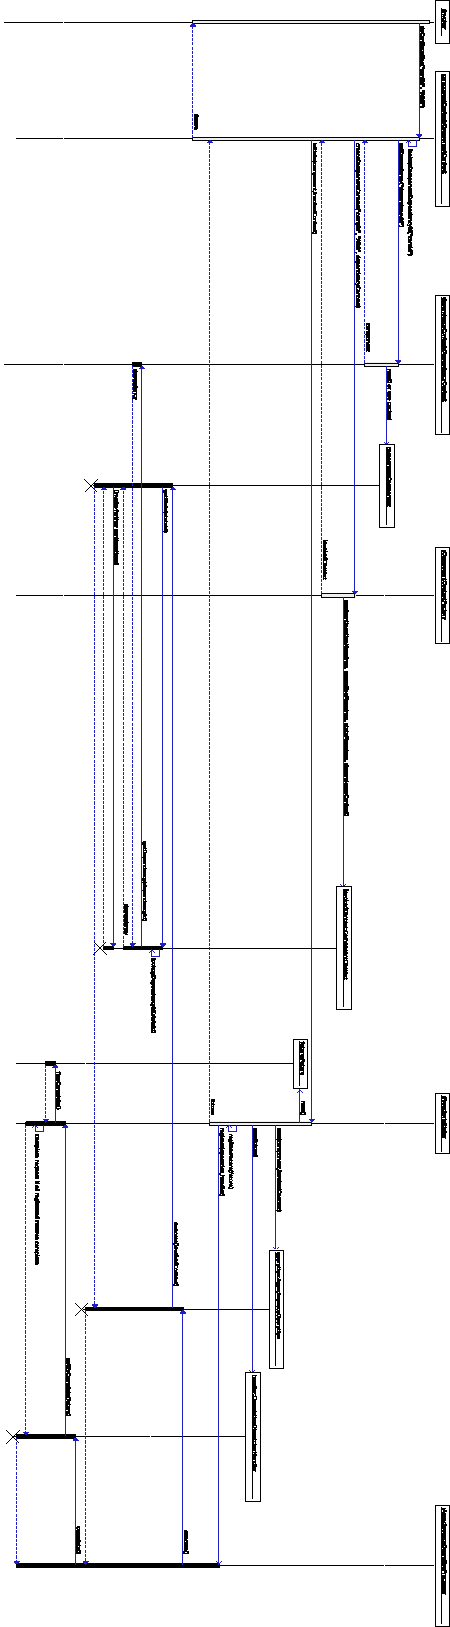
\includegraphics[width=6in]{DoContinuationSequenceDiagram}
\caption{Sequence diagram of invoking \texttt{doHandOff(\ldots)}.}
\label{fig:DoContinuationSequenceDiagram}
\end{figure}

The hand-off triggers the \texttt{TaskExecutor} to register a Task with a thread
pool for asynchronous execution.  A Future is returned from this registration to
notify when the Task is completed (\textsc{task complete}).  On completion of
the Task, the \texttt{TaskExecutor} is also notified of completion of the Task.
This allows the \texttt{TaskExecutor} to re-register any Tasks waiting on the
Future (\textsc{pick up task again}).  Tasks register for being picked up again
by the \texttt{continueTask()} method (Listing
\ref{lst:TaskCollaborationInterfaces}).

The tasks are constructed via the \textsc{dependency injection} pattern
\cite{ioc}.  The \texttt{Dependency\-InjectionFactory} (Listing
\ref{lst:TaskCollaborationInterfaces}) centrally manages the dependency
configuration and creates a \texttt{Depend\-ency\-Context} that constructs and
caches dependency instances for the tasks.  The \texttt{Dependency\-Context},
that manages the life-cycle of dependencies, is aligned to the
\texttt{TaskExecutor} life-cycle.  This allows for both the dependencies of the
tasks and the tasks themselves to be specific to the request being serviced.
As the dependencies are re-used across tasks, this allows tasks to share state
(\textsc{record information}).

The \texttt{doHandOff(\ldots)} does allow one argument to be passed to the
invoked component (\textsc{complete the form}).  This is for more intuitive
development by associating the invocation with passing state.  If multiple
arguments are required, they should be encapsulated into an object for passing.
To maintain loose coupling, the invoked task obtains the argument as state (i.e.
\texttt{getState(\ldots)} method in listing
\ref{lst:TaskCollaborationInterfaces}) so the invoked task need not
differentiate between dependencies and parameters (\textsc{record information}).
The invoked task may also ignore the hand-off argument should it not depend on
it.

The hand-off may borrow the thread of the invoking task if it results in being
executed by the same thread pool.  Rather than dispatching the task back to the
same thread pool, the \texttt{TaskExecutor} may borrow the thread to avoid the
overhead of a thread-context switch (\textsc{do your work}).

Exceptions from the methods are handled by being mapped to a \texttt{handOffId}.
 The task invokes the \texttt{handle\-Excep\-tion(\ldots)} method with the
exception.  The \texttt{handleException(\ldots)} method is implemented by
mapping the exception type to a \texttt{handOffId} and invoking the
\texttt{doHandOff(\ldots)} method with the exception as the argument
(\textsc{escalation}).  Hand-offs for specific exception types of the task may
be configured by the developer (\textsc{define process flows}).  The developer
will also configure ''catch all'' hand-offs for the application to handle
exceptions from any task to ensure all exceptions are handled (e.g. handling of
the runtime non-checked exceptions).

Integrating with code not contained in tasks does not allow access to the
\texttt{TaskContext} to invoke the hand-off for the first task.  The
\texttt{Process} (Listing \ref{lst:TaskCollaborationInterfaces}) provides an
interface that allows code not contained in a task to invoke the first task.
The returned \texttt{Future}, from the \texttt{TaskExecutor} tracking of tasks,
indicates when all tasks of the process are complete.  To retrieve results, the
\texttt{parameter} would be used as a visitor (\textsc{visitor} pattern
\cite{gof}) and be loaded with results by the invoked tasks.  The
\texttt{initialTaskId} may be mapped to a unique URL for external triggering of
the process (\textsc{contact us}).



\subsubsection*{Example}

Listing \ref{lst:Example_Method_Task} shows example method for retrieving
data from a cache.  The task for the \texttt{retrieve\-Data(\ldots)} method will:
\begin{enumerate}
  \item Obtain an instance of the \texttt{CacheOperation} via the \texttt{getState(\ldots)} method.
  \item Obtain both the \texttt{key}\footnote{\texttt{key} is a hand-off argument from the previous task.} and \texttt{cache} again via the \texttt{getState(\ldots)} method.
  \item Instantiate a proxy implementation of the \texttt{CacheHandOffs} interface that implements the \texttt{cacheMiss(\ldots)} method by invoking the \texttt{doHandOff(\ldots)} method. 
  \item Reflectively invokes the \texttt{retrieveData(\ldots)} method with the above arguments.
\end{enumerate}

\lstset{caption=Example developer code of a task for retrieving data from a cache\protect\footnotemark}
\begin{lstlisting}[float,label=lst:Example_Method_Task]

  interface CacheHandOffs {
    void cacheMiss(String key);
  }

  class CacheOperation {    
    public Data retrieveData(String key, Cache cache
                            , CacheHandOffs handOffs
                            ) throws IOException {
        Data data = cache.get(key);
        if (data == null) {
            handOffs.cacheMiss(key);
            return null; // finish operation
        }
        return data;
    }
  }
\end{lstlisting}
\footnotetext{\texttt{retrieveData} may also be a function should the implementing programming language support functions.}

Hand-offs from the \texttt{retrieveData(\ldots)} method are:
\begin{itemize}
  \item \texttt{cacheMiss(\ldots)} which is mapped to task to retrieve data from the database.
  \item Implicit hand-off which is mapped to the next task in the process\footnote{The return value from the method is used as the hand-off argument.}.
  \item \texttt{IOException} which is mapped to a task providing an error message page.  It may also be mapped to a task to retrieve the data from a database to attempt to continue servicing the request.
\end{itemize}


\subsubsection*{Consequences}

The mapping of \texttt{handOffId} to \texttt{taskId} (task) is contained within
configuration.  This enables changing the handling task without changing the
code of the methods.  Changing the handling task enables re-ordering the chained
sequence of tasks that are executed to service a request.  It also enables
configuring which method is invoked for each hand-off.  This removes the
hard-coding by the \textsc{proactor} pattern.   Furthermore, each invoked method
is undertaken by a thread from its responsible thread pool (i.e.
potentially different thread).  This removes the thread of control constraint
imposed by the \textsc{thread-per-request} pattern.

Understanding the collaboration of tasks would become difficult due to the
indirection involved.  The \textsc{define process flows} configuration, however,
provides means for graphical tools to manage the configuration to reduce this
difficulty.  The tools graphically represent the tasks as nodes with the
hand-off mappings being directed lines between these nodes.  Due to the
similarity of this configuration with service orchestration, this graphical
configuration is identified as Task Orchestration.

Furthermore, as components are potentially executed by different threads of
control, the stack trace automatically provided by the
\textsc{thread-per-request} pattern no longer reflects the call hierarchy for
servicing a request.  This can make it more difficult to debug issues.  However,
the \texttt{TaskExecutor} records the tree of components invoked so that the
tree can be traversed back to the root to identify the sequence of hand-offs to
the task throwing the exception.  The whole tree can also be reported to aid the
developer in debugging the cause of the issue.

Functions may also be used in place of methods.  When implementing tasks with
functions, the functions will not be pure.  As state is shared between tasks by
mutable state within dependencies, functions will need to cause side effects
(mutate state) to share state with other tasks (functions).



\subsubsection*{Related implementations}

This is an implementation of the Actor Model \cite{actors} as it adheres
to the principles of the Actor Model.  The task is the actor.  The asynchronous
communication between tasks decouples the hand-off argument (message) from the
sending task (actor).  The \texttt{taskId} provides an address for a task
(actor).  The provided \texttt{handOffId}s restricts the tasks (actors) that may
be used.

The implementation is also a form of continuation-passing style
\cite{continuations}.  The hand-off can be considered a continuation, as it is a
''goto'' for executing another task with a different thread (stack).  The benefit
of providing hand-offs through a context object is that the task is free to
depend on as many hand-offs as necessary, and not what the caller provides.  It
also means that as the application evolves the task encapsulates potential
changes requiring different hand-offs.  The indirection allows managing these
changes as configuration changes rather than code changes.

An \textsc{do it yourself} pattern has similarities to a monadic thread
\cite{monadic-thread}.  The tasks can be considered nodes in the lazy trace of
the monadic thread.  The advantage of an this implementation\footnote{Beyond
Task Orchestration being easier for the developer to understand than monad
programming.} is that the \textsc{responsible team} pattern allows the execution
of blocking I/O nodes (tasks) to be prioritised.  Monadic threads can not
prioritise blocking I/O nodes as they know little about them and subsequently
execute them within a single thread pool.

\textbf{TODO:} see preious paper for further related implementations.



\section{Patterns for building processes}


\subsection{\textsc{\textbf{task defines itself}}}

\subsubsection*{Alternate name} \textsc{method inversion of control}.

\subsubsection*{Context} Within an Office the task itself will define its
dependencies and when aspects are no longer its responsibility.  Providing a
fixed set of dependencies and fixed set of hand-offs to a person to achieve a
task will, unless a very simple task, likely result in the task being
unsuccessful.  To be successful, the person executing the task will seek out the
required dependencies and other people necessary to complete the task
successfully.

Furthermore, when conditions change the task may require new dependencies and
new hand-offs.  Introducing these new dependencies and hand-offs should be
encapsulated by the task and not significantly impact its containing process.

The method signature is fixed by the caller of the method and not the
implementation of the method.  The caller provides all arguments (dependencies)
and indicates that the method must be completed by the caller's thread of
control\footnote{The invoked method may create new threads but unless the caller
provides reference to existing thread pools, the method will not be able to use
them).}.

\subsubsection*{Problem} Let the method implementation define the method
signature and continue to enable the caller to invoke the method as the method
signature changes.

\subsubsection*{Forces} The caller must:
\begin{itemize}
  \item identify the method by name,
  \item provide all arguments to the method,
  \item handle all exceptions from the method,
  \item execute the method with its thread of control.
\end{itemize}

\subsubsection*{Solution} Use \textsc{hand-off} and \textsc{complete the form}
to relieve the caller from coupling the method signature and \textsc{define
process flows}, \textsc{record information}, \textsc{escalation} and
\textsc{responsible team} (via \textsc{categorise task}) to allow the method
implementation to define the method signature.

\subsubsection*{Consequences} The caller is no longer coupled to the method
signature.  This allows the method signature to change without impacting the
caller.

\textsc{define process flows} is necessary to understand the flow of the
application code, as the call hierarchies can no longer be determined by method
signatures.

\subsubsection*{Related Patterns}



\subsection{\textsc{\textbf{process defines itself}}}

\subsubsection*{Alternate name} \textsc{inversion of control}.

\subsubsection*{Context} The process is constructed from tasks.  As the tasks
define themselves, the process is subject to the necessitities of its containing
tasks.  The process, therefore, becomes the sum of all the dependencies and
hand-offs of its containing tasks.

Furthermore, determining whether it is a task or whether it is a process involving
multiple tasks executed by differing responsible teams is typically not
initially known.  Initially this may be determined correctly.  However, over
time conditions may change that cause a task to become more complex requiring
it to be transformed into a process involving many tasks and many responsible
teams (or vice-versa being transformed from a complex process to a simpler task).

Triggering a process within in an office is no different to triggering a task.
Like the task, the caller of the process is decoupled from the process.  The
\textsc{complete the form} is undertaken and provided to the first task of the
process.  Similar to the task, the process will \textsc{escalate} issues and
will \textsc{hand-off} to other processes/tasks as necessary.

Therefore, within an office the process defines itself to achieve its
requirements.  The process is also interchangeable with a task depending on the
complexity of the functionality.

\subsubsection*{Problem} Let a process define itself and in defining itself
the process is to have a similar interface to a task to be interchangeable with
a task.

\subsubsection*{Forces} Adding new tasks to a process is similar to adding new
functionality to a method.  Adding new functionality to a method involves:
\begin{itemize}
  \item new dependencies for the method that need to be referenceable from the functionality,
  \item new exceptions that may occur from the functionality, and
  \item a different threading model to efficiently undertake the functionality. 
\end{itemize}

\subsubsection*{Solution} Represent the process as a task in the \textsc{define
process flows}.  The process is given its own \texttt{taskId} that maps to the
initial task of the process\footnote{The process may expose multiple
\texttt{taskId} to enable starting at different tasks within it.}.  All
hand-offs not mapped to a task within the process become the set of hand-offs
for the process (this includes \textsc{escalation}).  All dependencies of the
contained tasks (from \textsc{record information}) becomes the set of
dependencies for the process.

To reduce the set of dependencies for the process, the process defines objects
to fulfill dependencies for its contained tasks.  These fulfilled dependencies
would then not be included in the interface set of dependencies for the process.

Similarly to reduce the hand-offs for the interface to the process, hand-offs
from multiple contained tasks are mapped to a single hand-off exposed from the
process.

\subsubsection*{Consequences} As the process is interchangeable with a task,
composite processes are built from other processes.  The interface of a
composite process is created in the same way as if it contained tasks.

Having composite processes constructed from other composite processes requires
the graphical representation of the \textsc{define process flows} pattern (Task
Orchestration) for the developer to understand the flows within the application.
 Adding composite processes adds further indirection that requires visual
representation to comprehend.

The \textsc{categorise task} pattern of each contained task within the process
(and composite processes) is still followed.  As the process is constructed from
only tasks, the process focuses only on functionality and allows all its tasks
to be executed by the \textsc{responsible team} pattern.  Therefore, if the
responsible thread pools are changed for the application the execution of the
tasks within the processes follow the new threading model without requiring code
changes.  This enables the threading model of the application to be tuned to the
hardware it is running on (e.g. single person team for a low powered single CPU
device or multiple specialised teams for high-performance multicore
hardware\footnote{Using increasingly better hardware follows the analogy of
growing the workforce of a business.  The business starts out only as a small
number of people doing many categories of tasks to becoming a large number of
people doing very specific categories of tasks.}).

\subsubsection*{Related Patterns}



\subsection{\textsc{\textbf{automate only where appropriate}}}

\subsubsection*{Alternate name} \textsc{evolve architecture}.

\subsubsection*{Context} Automating all processes is costly to a business.  In
many cases, using manual processes is cheaper than the cost of automating them.
 Furthermore, all processes may not be mature enough to be automated.
 
Automating a process requires standardising the process, ensuring the
dependencies of the process are available and accessible, and catering to all the
exceptions that may occur within the process.

Designing a business top down forces all processes to be of at least
standardised maturity to understand their interrelationships within the whole of
the business.  Having to mature all processes to be standardised increases cost
and forces less mature processes to be standardised before they have been
proven.  As the processes inevitably mature within the business, they become
different to their forced up front standardisation.

Businesses, therefore, standardise their processes by re-use of proven
processes/tasks (bottom-up approach) and only automate where appropriate.

Designing technology systems top-down is, therefore, not in alignment to how
businesses evolve.

\subsubsection*{Problem} Design technology systems bottom-up.

\subsubsection*{Forces} The method puts the control at the higher-level layers
of the system design.  The higher-level layer caller tightly couples the method
signature that the lower-level layer components may implement.  The lower-level
layers may not change the method signature without refactoring the higher-level
layers due to this tight coupling.

\subsubsection*{Solution} Use \textsc{task defines itself} to only build proven
tasks and build only the standardised processes through \textsc{process defines
itself}.

\subsubsection*{Consequences} The design of technology systems automate only the
mature processes within the business.  The less mature processes are left
undefined until they mature in the business.

This bottom-up approach to designing systems aligns both to the business
maturing and also modern development methodologies.  Modern development
methodologies, such as Agile, evolve the architecture upwards based on providing
value back to the business.  Therefore, only the processes that provide value
back to the business are built leaving the remaining processes manual (except
where there is necessary information capture for the processes of value, i.e.
\textsc{record information}).

\subsubsection*{Related Patterns}



\subsection{Implementation of process building patterns}

\subsubsection*{Background}

Applications built with \textsc{layers} typically impose a top-down approach to
design.  ``The \textsc{layers} require and provide \textsc{explicit interfaces}
from and to each other, in a top-down manner, from the higher to the lower
\textsc{layers}'' \cite[p. 11]{ioc}.  The higher-level layer components (object
that wraps a method, i.e. Task) define the variation points that are
``predefined points in the control and data flow which allow for modifying and
extending a component's behaviour'' \cite[p. 5]{ioc}.  A top-down approach is
required, as the higher-level layers control what variation points may be
implemented by the lower-level layer components.

The components need to be composed within an architecture that is dictated by
the framework.  The framework ``will define the overall structure, its
partitioning into \ldots [components], the key responsibilities thereof, how the
\ldots [components] collaborate, and the thread of control'' \cite[p.26]{gof}.
Using the components within a framework, therefore, identifies the following
requirements of a component's \textsc{explicit interface}:
\begin{itemize}
  \item components must have a key responsibility;
  \item components must be able to collaborate with other components; and
  \item components require a thread of control.
\end{itemize}

The collaboration of components can further be defined as the following
requirements:
\begin{itemize}
  \item components must be able to invoke other components;
  \item components must be able to share state; and
  \item exceptions from components need to be handled.
\end{itemize}

Within frameworks, the method signature is the interface between components.
``The set of all [method] signatures defined by an object \ldots characterizes
the complete set of requests that can be sent to the object'' \cite[p. 13]{gof}.
As frameworks are composed of objects, the method signature defines the
interface between objects and subsequently components.

The method signature meets the requirements as it:
\begin{itemize}
  \item has a key responsibility identified by its name;
  \item may invoke other methods;
  \item shares state with other methods by arguments and return values;
  \item provides declaration of exceptions for handling; and
  \item can be executed by the thread of control\footnote{For a stateless component interface, thread local variables are to be avoided to not incur affinity to a thread.}.
\end{itemize}

The method interface is, however, subject to tight coupling.  The tight
coupling occurs from the invoking higher-level layer component having to:
\begin{itemize}
  \item define the method name;
  \item provide the necessary arguments;
  \item possibly use the return value;
  \item handle potential exceptions; and
  \item provide the thread of control to execute the method.
\end{itemize}

This tight coupling imposed by the method results in the hierarchical
\textsc{layers} architecture where variation points (\textsc{explicit
interfaces}) are controlled by the higher-level layers.  The higher-level layer
component provides a \textsc{template method} \cite{gof} which is the variation
point that lower-level layer components may extend.

Within a \textsc{layers} architecture having variation points defined by
\textsc{template method}s requires refactoring of the \textsc{template method}
to increase the variability of the lower-level layer components.  Increasing the
variability ``requires adapting the \textsc{explicit interfaces} between the
\textsc{layers} to stipulate the types of variation parameters'' \cite[p.
5]{ioc} to allow control over the lower-level layers by the higher-level layers.

Instead of attempting to define variation points at the higher-level layers to
cover all possible variations of the lower-level layers, control should be
inverted and given to the lower-level layers to define the variation points. 
However, given that \textsc{template methods} impose a top-down control over
variation points, another form of \textsc{explicit interface} is necessary for
lower-level layer components to provide bottom-up control over defining
variation points for the application.



\subsubsection*{Implementation}

\textsc{record information} enables the lower-level layer component to specify
the state (objects) it requires.  The lower-level layer component specifies its
required state (objects) via \texttt{stateId}s.  As the lower-level layer
retrieves its state via \textsc{dependency injection}~\cite{ioc}, the invoking
higher-level layer components need only provide the single optionally used
argument.  This allows the lower-level layer component to specify as many
dependencies as is necessary.  It, therefore, gives the lower-level layer
component control over what state (objects/dependencies) it may depend on.

\textsc{categorise task} enables the lower-level layer component to specify its
thread of control.  By the the lower-level layer component having control over
specifying its required dependency types, the lower-level layer component may
specify additional dependencies to control which thread pool will be used to
execute it.

\textsc{hand-off} enables the lower-level layer component to specify its
required collaboration by \texttt{handOffId}s.  The mapping of
\texttt{handOffId} to \texttt{taskId} (\textsc{define process flows}) enables
configuring the higher-level layer components for handling each required
hand-off by the lower-level layer component.  As the invoking higher level-layer
component does not need to provide references to these handling components on
invoking the lower-level layer component, the lower-level layer component may
specify as many hand-offs as are necessary for its required collaboration
variation points.  This gives the lower-level layer component control over its
collaboration variation points.

Exceptions from components are handled by \textsc{escalation}.  The
exception is mapped to a \texttt{handOffId} and subsequently mapped to a
handling component.  As the invoking higher-level layer component is decoupled
from having to handle the exceptions, the lower-level layer component is free to
control throwing as many exceptions as is warranted.

Using the Office patterns provides the necessary inversion of control over
variation points as the lower-level layer component (Task) controls:
\begin{itemize}
  \item its name (\texttt{taskId}) which is decoupled from the invoking higher-level layer component invocation (\texttt{handOffId}) by \textsc{define process flows};
  \item which invocations (\texttt{handOffId}s) are necessary via \textsc{hand-off};
  \item what state (\texttt{stateId}s) is required by \textsc{record information};
  \item the types of exceptions that may be thrown by \textsc{escalation}; and
  \item the thread of control by \textsc{categorise task} specifying the \textsc{responsible team}.
\end{itemize}

Therefore, the \texttt{Task} interface (Listing
\ref{lst:TaskCollaborationInterfaces}) is the \textsc{explicit interface} of a
component that provides inversion of control to the method signature
(\textsc{task defines itself}).

To manage the complexity of the application's functionality, composite
components encapsulate complexity to enable more abstract management of the
application's functionality.  The \textsc{process defines itself} encapsulates
the complexity of composing tasks into more composite components (processes).

Futhermore, the top-down approach to designing an application requires a divide
and conquer approach over the entire scope of the application requirements.
Without understanding all the complexities, the design may not adequately meet
the business needs and require significant refactoring to align to business
needs.  Building only the mature processes (\textsc{automate only where
appropriate}) removes the need to understand all complexities as only
understanding of the scope of each process is required.


\subsubsection*{Consequences}

Within \textsc{task defines itself}, object-orientation provides the implicit
state (dependencies) to a task.  Explicit dependencies are injected as arguments
into the method (\textsc{record information}).  Object-orientation implicitly
provides the instance/class references to the method.  Having implicit
references tightly couples the tasks and should be avoided in implementing
tasks.  Furthermore, as the application behaviour is implemented in tasks via
methods, the application is no longer constructed only as a graph of
collaborating hierarchical objects.

Using \textsc{process defines itself} enables bottom-up control over the design
of the application.  As the variation points are controlled by the tasks,
developers may start by building the tasks first.  As the tasks are less
abstract, the developer is able to focus on more concrete problems and provide
only the necessary variation points to solve the particular problem.  This
avoids over engineering the design of the application.  Furthermore, as the
processes are built last, there is less need for large initial top-down designs.

\textsc{process defines itself} also enables bottom-up evolution of the
application.  Within applications imposing top-down design, the
\textsc{explicit interface} (\textsc{template method}) between \textsc{layers}
needs to be refactored to account for required changes to increase the
variability of the lower-level layer components as the application evolves
\cite{ioc}.  Within bottom-up \textsc{process defines itself}, the tasks may
introduce new variation points that are implemented by \textsc{define process
flows} and \textsc{record information} of the higher-level processes and
composite processes.  As the \textsc{explicit interface} to invoke the
task/process does not change, the higher-level layer calling code does not
require refactoring to evolve the application.




\section{Conclusion}

The use of proven patterns occurring within an office has highlighted and
resolved limitations in existing middleware framework patterns.  The
\textsc{responsible team} pattern and its related task execution patterns
provides improved performance tuning of the application.  The \textsc{define
process flows} pattern and its related patterns decreases the coupling between
methods to enable more flexible change.  Finally, using these patterns together
for the \textsc{task defines itself} pattern and its related patterns provides
inversion of control to enable building application's bottom-up.

As this paper covers the implementation patterns of OfficeFloor, future work
will describe the usage patterns for developers to build applications with
OfficeFloor.



\section*{Acknowledgment} 

I thank my wife Melanie for her patience and support
of me developing OfficeFloor on top of my day job.  If she was anyone else
OfficeFloor would not have been built and this work would not have resulted from
OfficeFloor.  I also thank my good friend Matthew Brown for being a sounding
board to many of my ideas.

I am also grateful for the wise shepherding by Veli-Pekka Eloranta and the
feedback from the participants of EuroPlop 2013.


\bibliographystyle{style/acmlarge}
\bibliography{tici}

\end{document}
